\begin{flushleft}

	\bigskip
		\begin{enumerate}
			\item (Re)boot the system.
			\item Interrupt the boot loader menu countdown by pressing any key.
			\item Move the cursor to the entry to be started.
			\item \textbf{Press e} to edit the current entry.
			\item Move the cursor to the line that starts with \textbf{linux}. This is the kernel command line.
			\item Append \textbf{systemd.unit=desired.target}.
			\newline eg: systemd.unit=multi-user.target
			
			\begin{figure}[h!]
				\centering
				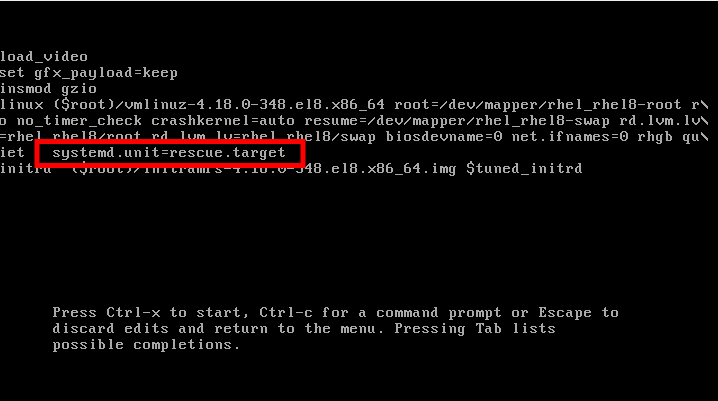
\includegraphics[scale=.5]{content/chapter1/images/rescue.png}
				\caption{Sample output}
				\label{fig:free_h_s_2}
			\end{figure}
			
			\item Press \textbf{Ctrl+x} to boot with these changes.
		\end{enumerate}
	
\end{flushleft}

\newpage